%% last updated in April 2002 by Antje Endemann
%% Based on CVPR 07 and LNCS, with modifications by DAF, AZ and elle, 2008 and AA, 2010, and CC, 2011; TT, 2014; AAS, 2016
%
%%\documentclass[runningheads]{llncs}
%%\usepackage{graphicx}
%%\usepackage{amsmath,amssymb} % define this before the line numbering.
%%%\usepackage{ruler}
%%\usepackage{color}
%%\usepackage[width=122mm,left=12mm,paperwidth=146mm,height=193mm,top=12mm,paperheight=217mm]{geometry}
%
%
%%\begin{document}
%%% \renewcommand\thelinenumber{\color[rgb]{0.2,0.5,0.8}\normalfont\sffamily\scriptsize\arabic{linenumber}\color[rgb]{0,0,0}}
%%% \renewcommand\makeLineNumber {\hss\thelinenumber\ \hspace{6mm} \rlap{\hskip\textwidth\ \hspace{6.5mm}\thelinenumber}}
%%% \linenumbers
%%\pagestyle{headings}
%%\mainmatter
%%\def\ECCV18SubNumber{1000}  % Insert your submission number here
%%
%%\title{} % Replace with your title
%%
%%\titlerunning{ECCV-18 submission ID \ECCV18SubNumber}
%%
%%\authorrunning{ECCV-18 submission ID \ECCV18SubNumber}
%%
%%\author{}
%%\institute{}
%%
%%
%%%\maketitle
%%
%%\section*{Appendix A: Solvers}
%%We reproduce our optimization problem below for reference:
%%\begin{equation}
%%\begin{aligned}
%%\min_{\amap, \bmap} ~ &\big\| \dfilter\mask\odot\big(\ic-\bayer\big(\amap \odot \iref+ \bmap \odot (\ones-\iref)\big) \big) \big\|_2^2 \\
%%+ &\lambda_{1} \|\edgemask\odot\nabla\amap\|_{1} + \gamma_{1}\sum_{l\neq k}\| \nabla\amap_{l}\odot \amap_{k} - \nabla\amap_{k}\odot \amap_{l} \|_1  \\
%%+ &\lambda_{2} \|\edgemask\odot\nabla\bmap\|_{1} + \gamma_{2}\sum_{l\neq k}\| \nabla\bmap_{l} - \nabla\bmap_{k} \|_1 ~.
%%\end{aligned}
%%\end{equation}
%%where $\amap, \bmap, \iref, \edgemask \in \mathbb{R}^{3n}$ and $\ic, \mask \in \mathbb{R}^{n}$ are in the vectorized form with $n$ being the total number of pixels. $\bayer \in \mathbb{R}^{n\times 3n}$ denotes the Bayer downsampling matrix, $\dfilter \in \mathbb{R}^{n\times n}$ is a convolution matrix representing a Gaussian filter, and $\nabla$ denotes the gradient operator for the underlying images. 
%%
%%Writing $\latent = \begin{bmatrix}
%%\amap; & \bmap
%%\end{bmatrix} \in \mathbb{R}^{6n}$ and expressing the element-wise multiplication as matrix multiplication with a diagonal matrix, the above problem can be reformulated as 
%%\begin{equation}
%%\begin{aligned}
%%\min_{\latent} ~ f(\latent) + g(\priormatrix \latent)
%%\end{aligned}
%%\label{eqn:optimization}
%%\end{equation}
%%where $f(\latent) = \big\| \dfilter\diag{\mask}\big(\ic-\bayer \begin{bmatrix}
%%\diag{\iref}~ &  \diag{\ones-\iref}
%%\end{bmatrix} \latent  \big) \big\|_2^2$ and $g(\cdot) = \big\| \cdot \big\|_{1}$ with $\diag{\mathbf{V}}$ representing a diagonal matrix with diagonal entries given by a vector $\mathbf{V}$. The combined matrix $\priormatrix$ is obtained by stacking the component matrices. More specifically, 
%% \begin{equation}
%%\priormatrix = \begin{bmatrix}
%%\lambda_{1}\diag{\edgemask}\nabla~ &  \zeros \\
%%\zeros~ &  \lambda_{2}\diag{\edgemask}\nabla \\
%%\gamma_{1} \ccamatrix &  \zeros \\
%%\zeros &  \gamma_{2} \ccbmatrix
%%\end{bmatrix}.
%%\end{equation}
%%where $\ccamatrix$ and $\ccbmatrix$ compute the difference between (scaled) gradients of different channels of $\amap, \bmap$ respectively.
%%
%%The minimization problem \eqref{eqn:optimization} is of the standard form where a number of non-linear solvers can be directly applied. In the paper we have used the linearized ADMM algorithm with steps included below for completeness.
%%\begin{algorithm}[H]
%%\begin{algorithmic}[1]
%%	\caption{Linearized ADMM} \label{tab:ADMM}
%%	\Input $\iref, \ic$; Parameters $\mu, \alpha$ satisfying $0<\mu \le \alpha/\|\priormatrix\|_{2}$.
%%	\item[Repeat until convergence:]
%%	\State $\latent^{k+1} = \underset{\latent}{\text{argmin}}~ f(\latent) + \frac{1}{2\mu}\big\|\latent - \big( \latent^{k}-\frac{\mu}{\alpha}\priormatrix^{T}(\priormatrix\latent^{k}-\mathbf{z}^{k}+\mathbf{u}^{k} ) \big) \big\|_2^2$~,
%%	\State $\mathbf{z}^{k+1} = \underset{\mathbf{z}}{\text{argmin}}~ g(\mathbf{z})+ \frac{1}{2\alpha}\big\| \mathbf{z} - (\priormatrix \latent^{k+1}+\mathbf{u}^{k}) \big\|_2^2 $~,
%%	\State $\mathbf{u}^{k+1} = \mathbf{u}^{k} + \priormatrix\latent^{k+1} - \mathbf{z}^{k+1}$~.
%%	\Output $\latent^{*} = \begin{bmatrix}
%%	\amap^{*}; & \bmap^{*}
%%	\end{bmatrix}$ and $\iout = \amap^{*} \odot \iref+ \bmap^{*} \odot (\ones-\iref)$.
%%\end{algorithmic}
%%\end{algorithm}
%%
%%\clearpage
%%
%%\end{document}
%
%
%
%\documentclass[10pt,twocolumn,letterpaper]{article}
%
%\usepackage{cvpr}
%\usepackage{times}
%\usepackage{epsfig}
%\usepackage{graphicx}
%\usepackage{amsmath}
%\usepackage{amssymb}
%\usepackage[normalem]{ulem}
%

%
\newcommand{\ic}[0]{\mathbf{I^{\text{cfa}}}}
\newcommand{\iref}[0]{\mathbf{I^{\textrm{ref}}}}
\newcommand{\iout}[0]{\mathbf{I^{\textrm{out}}}}
\newcommand{\ifinal}[0]{\mathbf{I^{\textrm{final}}}}
\newcommand{\ones}[0]{\mathbf{1}}
\newcommand{\zeros}[0]{\mathbf{0}}
\newcommand{\amap}[0]{\mathbf{A}}
\newcommand{\bmap}[0]{\mathbf{B}}
\newcommand{\bayer}[0]{\mathbf{D}}
\newcommand{\mask}[0]{\mathbf{W}}
\newcommand{\dfilter}[0]{\mathbf{H}}
\newcommand{\edgemask}[0]{\mathbf{E}}
\newcommand{\prior}[1]{\mathbf{\Phi{(#1)}}}
\newcommand{\latent}[0]{\mathbf{x}}
\newcommand{\priormatrix}[0]{\mathbf{K}}
\newcommand{\ccamatrix}[0]{\mathbf{K_{A}}}
\newcommand{\ccbmatrix}[0]{\mathbf{K_{B}}}
\newcommand{\diag}[1]{\text{diag}_{#1}}
%
%% Include other packages here, before hyperref.
%
%% If you comment hyperref and then uncomment it, you should delete
%% egpaper.aux before re-running latex.  (Or just hit 'q' on the first latex
%% run, let it finish, and you should be clear).
%\usepackage[pagebackref=true,breaklinks=true,letterpaper=true,colorlinks,bookmarks=false]{hyperref}
%
%% \cvprfinalcopy % *** Uncomment this line for the final submission
%
%\def\cvprPaperID{****} % *** Enter the CVPR Paper ID here
%\def\httilde{\mbox{\tt\raisebox{-.5ex}{\symbol{126}}}}
%
%
%
%% Pages are numbered in submission mode, and unnumbered in camera-ready
%\ifcvprfinal\pagestyle{empty}\fi


\documentclass{bmvc2k}

\usepackage{algorithmicx}
\usepackage{algorithm}
\usepackage{algpseudocode}



\algnewcommand\algorithmicinput{\textbf{Input:}}
\algnewcommand\algorithmicoutput{\textbf{Output:}}
\algnewcommand\Input{\item[\algorithmicinput]}
\algnewcommand\Output{\item[\algorithmicoutput]}

%% Enter your paper number here for the review copy
\bmvcreviewcopy{xx}

\title{Author Guidelines for the\\ British Machine Vision Conference}

% Enter the paper's authors in order
%\addauthor{Name}{email/homepage}{INSTITUTION_CODE}
\addauthor{Susan Student}{http://www.vision.inst.ac.uk/~ss}{1}
\addauthor{Petra Prof}{http://www.vision.inst.ac.uk/~pp}{1}
\addauthor{Colin Collaborator}{colin@collaborators.com}{2}

% Enter the institutions
% \addinstitution{Name\\Address}
\addinstitution{
	The Vision Institute\\
	University of Borsetshire\\
	Wimbleham, UK
}
\addinstitution{
	Collaborators, Inc.\\
	123 Park Avenue,\\
	New York, USA
}

\runninghead{Student, Prof, Collaborator}{BMVC Author Guidelines}

% Any macro definitions you would like to include
% These are not defined in the style file, because they don't begin
% with \bmva, so they might conflict with the user's own macros.
% The \bmvaOneDot macro adds a full stop unless there is one in the
% text already.
\def\eg{\emph{e.g}\bmvaOneDot}
\def\Eg{\emph{E.g}\bmvaOneDot}
\def\etal{\emph{et al}\bmvaOneDot}

%----------------
\begin{document}
	
	%%%%%%%%% TITLE
	\title{Robust Joint Image Reconstruction from Color and Monochrome Cameras}
	
	\author{First Author\\
		Institution1\\
		Institution1 address\\
		{\tt\small firstauthor@i1.org}
		% For a paper whose authors are all at the same institution,
		% omit the following lines up until the closing ``}''.
		% Additional authors and addresses can be added with ``\and'',
		% just like the second author.
		% To save space, use either the email address or home page, not both
		\and
		Second Author\\
		Institution2\\
		First line of institution2 address\\
		{\tt\small secondauthor@i2.org}
	}
	
\section*{Appendix A: Solver}
	We reproduce our optimization problem below for reference:
\begin{equation}
	\begin{aligned}
	\min_{\amap, \bmap} ~ &\big\| \ic-\bayer\big(\amap \odot \iref+ \bmap \odot (\ones-\iref)\big) \big\|_2^2 \\
	+ &\lambda_{1} \|\mask\odot\nabla\amap\|_{1} + \lambda_{2} \|\mask\odot\nabla\bmap\|_{1}  \\
	+ &\gamma_{1}\sum_{l\neq k}\| \mask\odot(\nabla\amap_{l}\odot \amap_{k} - \nabla\amap_{k}\odot \amap_{l}) \|_1 \\
	+ &\gamma_{2}\sum_{l\neq k}\| \mask\odot(\nabla\bmap_{l} - \nabla\bmap_{k}) \|_1,
	\end{aligned}
\end{equation}
where $\amap, \bmap, \iref \in \mathbf{R}^{3n}$ and $\ic \in \mathbf{R}^{n}$ are in the vectorized form with $n$ being the total number of pixels. $\bayer \in \mathbf{R}^{n\times 3n}$ denotes the Bayer downsampling matrix. $\nabla$ denotes the gradient operator for the underlying images and $\mask$ is a per-pixel weight matrix that matches the output dimension of $\nabla$. 
	
Writing $\latent = \begin{bmatrix}
\amap; & \bmap
\end{bmatrix} \in \mathbf{R}^{6n}$ and expressing the element-wise multiplication as matrix multiplication with a diagonal matrix, the above problem can be reformulated as 
\begin{equation}
\begin{aligned}
&\min_{\latent} ~ f(\latent) + g(\priormatrix \latent),
\end{aligned}
\label{eqn:optimization}
\end{equation}
with $f(\latent) = \big\| \ic-\bayer \begin{bmatrix}
\diag{\iref} \quad  \diag{\ones-\iref}
\end{bmatrix} \latent   \big\|_2^2$ and $g(\cdot) = \big\| \cdot \big\|_{1}$. Here $\diag{\mathbf{v}}$ represents a diagonal matrix with diagonal entries given by a vector $\mathbf{v}$. The combined matrix $\priormatrix$ is obtained by stacking the component matrices. More specifically, 
 \begin{equation}
\priormatrix = \begin{bmatrix}
\lambda_{1}\diag{\mask}\nabla~ &  \zeros \\
\zeros~ &  \lambda_{2}\diag{\mask}\nabla \\
\gamma_{1} \ccamatrix &  \zeros \\
\zeros &  \gamma_{2} \ccbmatrix
\end{bmatrix},
\end{equation}
where $\ccamatrix$ and $\ccbmatrix$ compute the difference between (scaled) gradients of different channels of $\amap, \bmap$ respectively.
	
	The minimization problem \eqref{eqn:optimization} has a
        standard form for which a number of non-linear solvers are
        available. In our implementation we have used the linearized ADMM algorithm with steps included below for completeness.
	\begin{algorithm}[H]
		\begin{algorithmic}[1]
			\caption{Linearized ADMM} \label{tab:ADMM}
			\Input $\iref, \ic$; Parameters $\mu, \alpha$ satisfying $0<\mu \le \alpha/\|\priormatrix\|_{2}$.
			\item[Repeat until convergence:]
			\State $\latent^{k+1} = \underset{\latent}{\text{argmin}}~ f(\latent) + \frac{1}{2\mu}\big\|\latent - \big( \latent^{k}-\frac{\mu}{\alpha}\priormatrix^{T}(\priormatrix\latent^{k}-\mathbf{z}^{k}+\mathbf{u}^{k} ) \big) \big\|_2^2$~,
			\State $\mathbf{z}^{k+1} = \underset{\mathbf{z}}{\text{argmin}}~ g(\mathbf{z})+ \frac{1}{2\alpha}\big\| \mathbf{z} - (\priormatrix \latent^{k+1}+\mathbf{u}^{k}) \big\|_2^2 $~,
			\State $\mathbf{u}^{k+1} = \mathbf{u}^{k} + \priormatrix\latent^{k+1} - \mathbf{z}^{k+1}$~.
			\Output $\latent^{*} = \begin{bmatrix}
			\amap^{*}; & \bmap^{*}
			\end{bmatrix}$ and $\iout = \amap^{*} \odot \iref+ \bmap^{*} \odot (\ones-\iref)$.
		\end{algorithmic}
	\end{algorithm}
	
\section*{Appendix B: Implementation Details of W-Matrix Reconstruction }

The flow consistency is measured for
each pixel by checking if its L2 distance between forward and backward
flows is below $2$ pixels. 

The visual similarity is evaluated	between the reference image and the green channel of color images used in alignment. 
Texture similarity can be identified by comparing SIFT descriptor \cite{Lowe:2004:SIFT} on gradient images.
If the L1-norm SIFT difference of two aligned pixels is less than $\lambda_{sift}=2$, the two pixels are
identified to be visually similar and thus reliably aligned. 
Before computing the SIFT descriptor, the image gradients are smoothed by
guided filter~\cite{He:2013:GIF} with a window size of $4$ pixels and
$0.03$ degree of smoothing. 
Two textureless regions can also be perceived as being similar to each other,  if both of their local gradients are smaller than a threshold of $0.06$.

For detecting occluded pixels, the difference between image edge maps is evaluated with structural similarity (SSIM) \cite{Wang:2004:IQA} in which only the structure comparison module is used. 
The two aligned
	pixels are deemed unreliable if the SSIM is smaller than $0.3$.  The
	image edge is detected via SDE detector \cite{Dollar:2013:SDE}, which
	is also used in EpicFlow
	\cite{revaud:2015:FLOW}. But edge-based
	detection cannot deal with relatively large occluded regions.  Additionally, flow gradients are used to detect large occluded regions. In a
	two-camera stereo system, where the monochrome camera is fixed to
	always be located either on the left or on the right of the RGB
	camera, occlusion artifacts always appear on the same side of an
	object boundary. This means that, for a chosen camera, we only need to deal with 
	either positive or negative flow gradients. Therefore we
	first discard flow gradients with the unwanted sign depending on the
	camera position. Absolute values of gradients are used for subsequent
	processing.  The absolute gradients smaller than $0.5$ is set as
	$0$. We remove small non-zero region with a threshold of $100$
	pixels. This can remove flow gradients that result from miscalculated
	and noisy flow fields at, for example, textureless regions instead of
	at real depth discontinuities.  Then a 1-D Gaussian filter with
	standard deviation of $\sigma=40$ along x-axis is used to dilate the
	processed absolute gradient field. A pixel is occluded, if its dilated
	gradient exceed $0.1$ and the L2 distance between forward and backward flows 
	exceeds $15$ pixels. 
 	For highly regular-textured regions, 
	if L1 SIFT difference is smaller than $\Lambda_{sift}=5$, which is loosened from 
	$\lambda_{sift}=2$ and absolute flow gradient is smaller than $0.03$, the two 
	pixels are well-aligned.
	
	In this end, the 
	binary mask of reliable pixels are filtered using median filter with $15 \times 
	15$ windows to remove thresholding noise. In $\mask$-matrix, the excluded pixels 
	are given low weight, e.g.\ $0.05$, to ensure the reconstructed pixels are 
	similar to the upsampled raw pixels rather than the reference artifact pixels, 
	while encouraging reliable pixels to propagate $\amap$ and $\bmap$ to these 
	unreliable pixels.  The reliable pixels are set to have weight $1$. $\mask$ is 
	finally filtered by Gaussian filter with a standard deviation of $2$ pixels to 
	smoothen the boundaries.
	
	
\section*{Appendix C: Robustness of W-Matrix Construction }
Our algorithm is robust to underlying artifacts in the reference image. The $\mathbf{W}$-matrix is robustly and conservatively constructed through a relatively complete heuristic rules. We run our W-matrix construction algorithm with randomly and independently perturbed parameters on Middlebury dataset 2014. Once the image pair is aligned, we calculate PSNR on reliably and unreliably aligned pixels identified by the W-matrix, which is shown in Fig.~\ref{fig:robustness}  (Left). 
{We found that perturbing each parameter by an average of 20 \% (maximum 40 \%) has insignificant impact on reference images.

Even if some artifact pixels are wrongly weighted too high in the regularization term by $\mathbf{W}$, our algorithm still produces high-quality reconstruction results using a single set of parameters since our image formation model has considered underlying artifacts in the reference images. We do not assume the reference monochrome image is perfectly aligned to the color image. 
We run the perturbation experiments on datasets of our captured image pairs.  
Fig.~\ref{fig:robustness} (Right) shows the parameter perturbation has even less impact on the reconstructed images quality. The maximum and minimum PSNR of the reconstructed images are almost unchanged. 

%We also present some qualitative comparisons about the effect of the convolution in the data term and the weight matrix in the regularization term in Fig.~xxx and supplementary materials.

%All results (in the paper and the supplementary material) are obtained under a single set of $\mask$-matrix construction parameters.
	
	
	
\begin{figure}[htb]
		\centering
		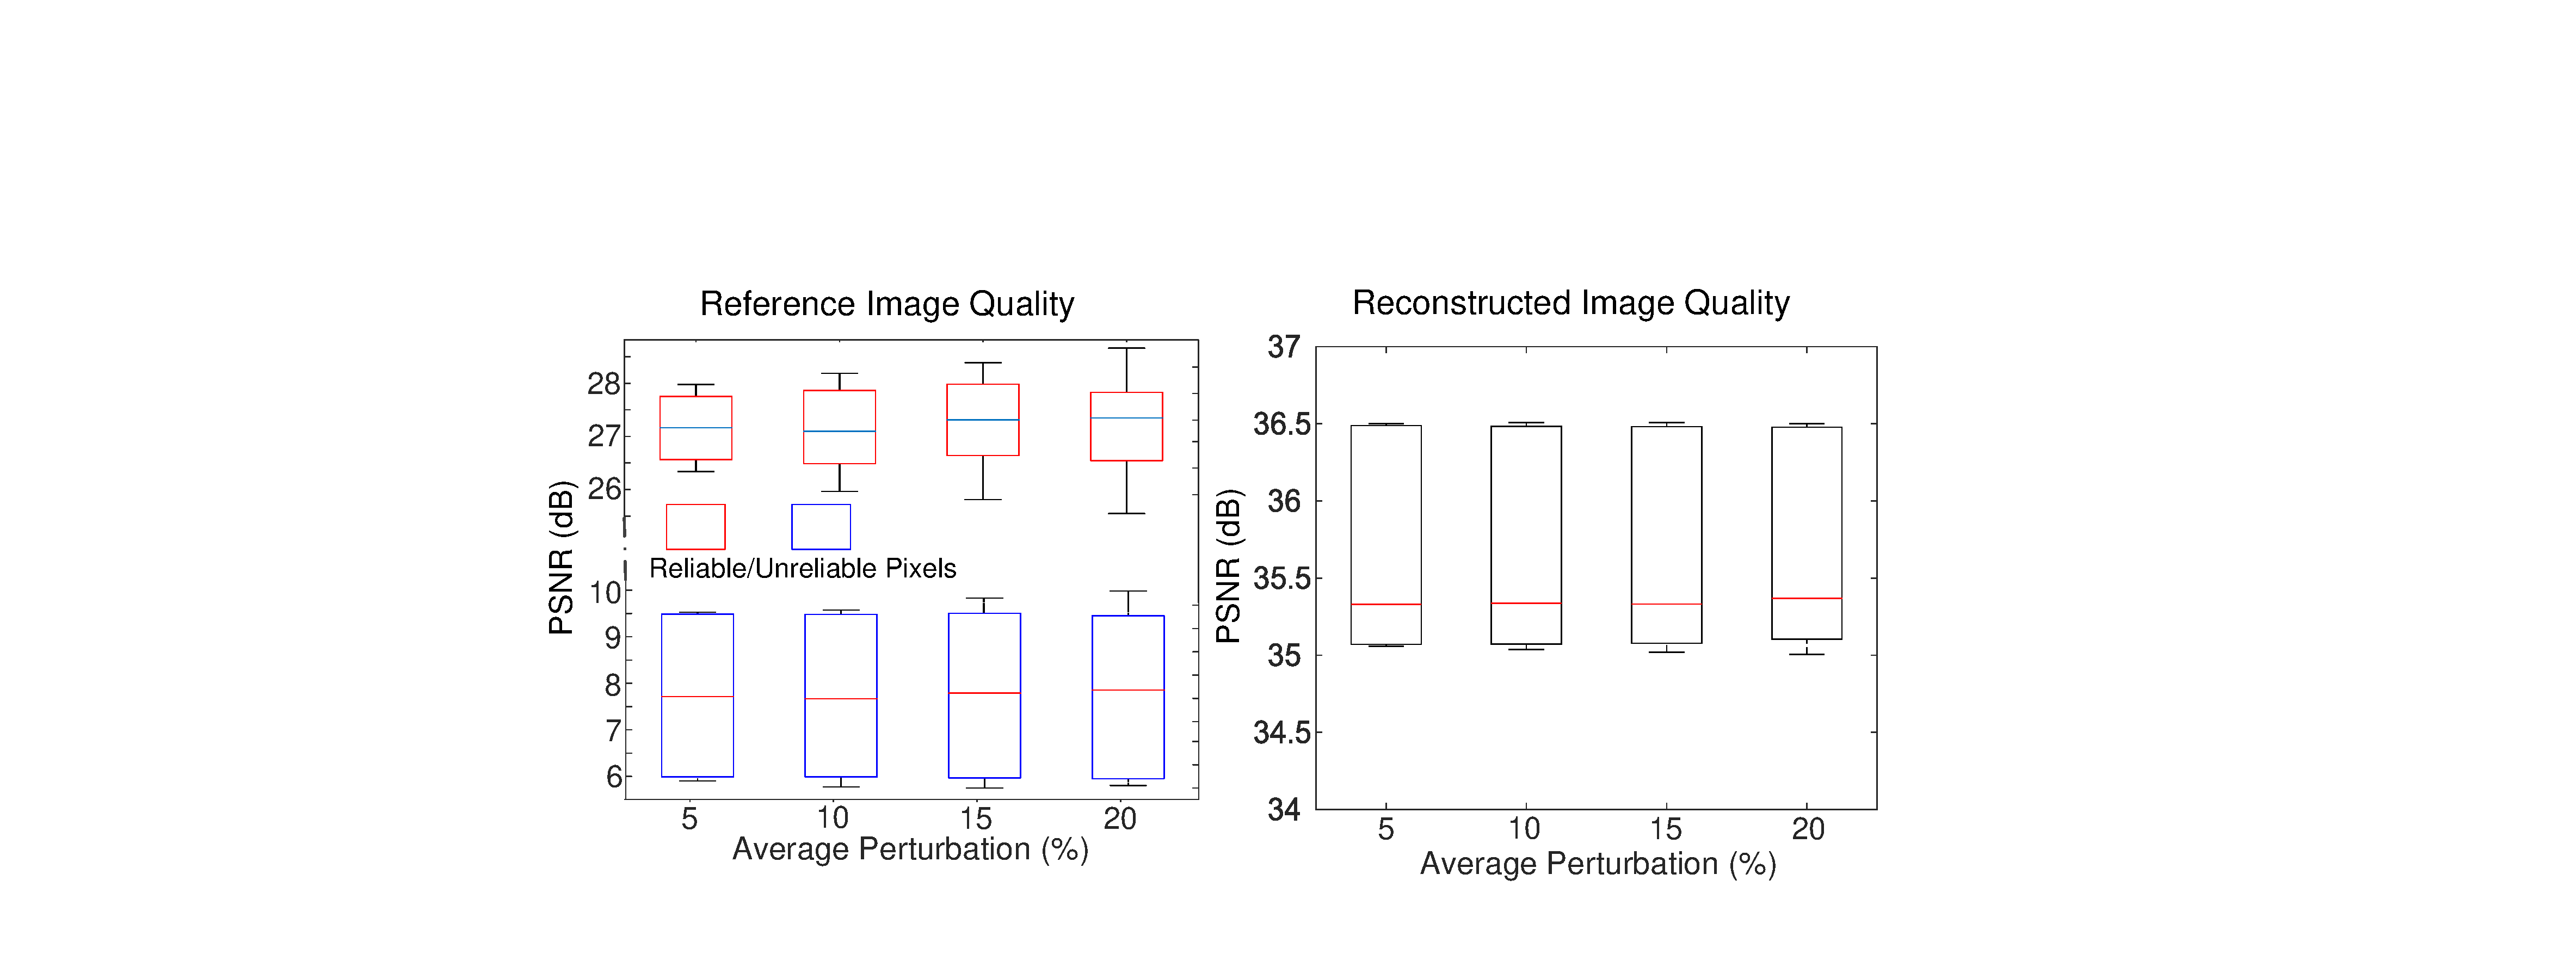
\includegraphics[width=0.8\textwidth]{perturbation.pdf}
		\caption{Box plot of PSNR with respect of parameter perturbation. Middle lines in the box indicate the mean, the upper and lower lines  indicate the maximum and minimum. The length of the box suggests PSNR variance.}
		\label{fig:robustness}
\end{figure}

	{\small
%	\bibliographystyle{ieee}
	\bibliography{egbib}
}
\end{document}






%\maketitle







